\section{Energiewissenschaften}
\subsection{Energieumwandlung von thermisch in elektrisch}
\noindent\textbf{1. Wie lautet der erste Hauptsatz der Thermodynamik?}\\
\begin{addmargin}[25pt]{0pt}
Der erste Hauptsatz der Thermodynamik ist der Energieerhaltungssaatz, er lautet:
\begin{equation}\label{eq:Energieerhaltung}
    \si{d}U = \delta Q + \delta W
\end{equation}
Dabei ist d$U$ die Änderung der inneren Energie des Systems, $\delta Q$ die zugeführte oder abgeführte Wärme und $\delta W$ die zugeführte oder abgeführte Arbeit. Die verschiedene Darstellung der einzelnen Differentiale hat dabei eine besondere Bedeutung, das totale Differential wie in d$U$ zeigt an dass die innere Energie $U$ eine Zustandsgröße ist. Zustandsgrößen sind nur von den aktuellen Kenngrößen des Systems abhängig unabhängig wie diese erreicht wurden. Zustandsgrößen sind wegunabhängig integrierbar. Das Differential $\delta$ zeigt Prozessgrößen an, diese sind nur sinnvoll definiert während einer Zustandsänderung und sie charakteriseren diese. Prozessgrößen haben kein totales Differential also können sie auch nicht wegunabhängig integriert werden.\\    
\end{addmargin}

\noindent\textbf{2. Was ist Exergie?}\\
\begin{addmargin}[25pt]{0pt}
Die Exergie ist ein Maß dafür wie nutzbar die innere Energie eines Systems ist. Sie ist definiert als die Arbeit die man maximal aus einem System entziehen kann wenn es es mit einer Carnot-Maschine mit der Umgebung verbindet. Die Exergie ist demnach eine von der Umgebung abhängige Zustandsgröße. Bei irreversiblen Prozessen, wie zum Beispiel der Wärmefluss von einem warmen Reservoir zu einem kalten Reservoir, wird Exergie übertragen, dahingegen ist die Exergie bei reversiblen Prozessen erhalten.\\
\end{addmargin}

\noindent\textbf{3. Was ist der Unterschied zwischen energetischem und exergetischem Wirkungsgrad?}\\
\begin{addmargin}[25pt]{0pt}
Der energetische Wirkungsgrad oder 1st law efficiency gibt Auskunft darüber wie viel Energie der gewünschten Form man aus einer Maschine erhält $E_{\si{out}}$ wenn man eine Menge $E_{\si{in}}$ einer ungewünschten Form in die Maschine eingibt der energetische Wirkungsgrad ist definiert als:
\begin{equation}\label{eq:energetischer_Wirkungsgrad}
    \eta_1 = \frac{E_{\si{out}}}{E_{\si{in}}}
\end{equation}
Andererseits ist der exergetische Wirkungsgrad oder 2nd law efficiency definiert als der Quotient aus Exergie nach dem Prozess und Exergie vor dem Prozess:
\begin{equation}\label{eq_exergetischer_Wirkungsgrad}
    \eta_2 = \frac{\Phi_{\si{out}}}{\Phi_{\si{in}}}
\end{equation}
Damit gibt $\eta_2$ Informationen darüber wie viel nutzbare Energie in nicht nutzbare Energie während eines Prozesses umgewandelt wird.\\
\end{addmargin}
\newpage
\noindent\textbf{4. Wie ändert sich die Exergie eines Systems A, wenn dieses System eine Wärmemenge $Q$ isotherm aufnimmt oder abgibt?}\\
\begin{addmargin}[25pt]{0pt}
Naiverweise könnte man annehmen, dass die Exergieänderung einfach der Wärme entspricht, dabei wurde aber ignoriert dass wenn das System A Wärme isotherm aufnimmt/abgibt es auch Arbeit an der Umgebung verrichtet. Diese Arbeit muss man ebenfalls in der Exergiebetrachtung berücksichtigen. Damit ergibt sich für die Exergieänderung des Systems A:
\begin{equation}\label{eq:Exergieänderung_A}
    \Phi_{\si{A}} = Q\cdot \left(1-\frac{T_{\si{am}}}{T_{\si{A}}}\right)
\end{equation}
Wobei $T_{\si{am}}$ die Umgebungstemperatur ist. Analog kann man den Exergieverlust bestimmen, wenn eine Wärme Q von einem System A auf ein System B übertragen wird und es gilt $T_{\si{A}} > T_{\si{B}} >T_{\si{am}}$. Der Gesamtexergieverlust ist dann:
\begin{equation}\label{eq:Exergieverlust}
    \left| \Phi_{\si{A}}\right| - \Phi_{\si{B}} = QT_{\si{am}}\left(\frac{1}{T_{\si{B}}}-\frac{1}{T_{\si{A}}}\right)
\end{equation}
\end{addmargin}

\noindent\textbf{5. Wie funktioniert eine Wärmepumpe?}\\
\begin{addmargin}[25pt]{0pt} 
Wärmepumpen nutzen elektrische Energie um Wärme von einem kalten Reservoir in ein warmes Reservoir zu pumpen. Ein Schema einer Wärmepumpe ist in Abbildung \ref{fig:heat_pump} gezeigt.
\begin{figure}[h]
    \centering
    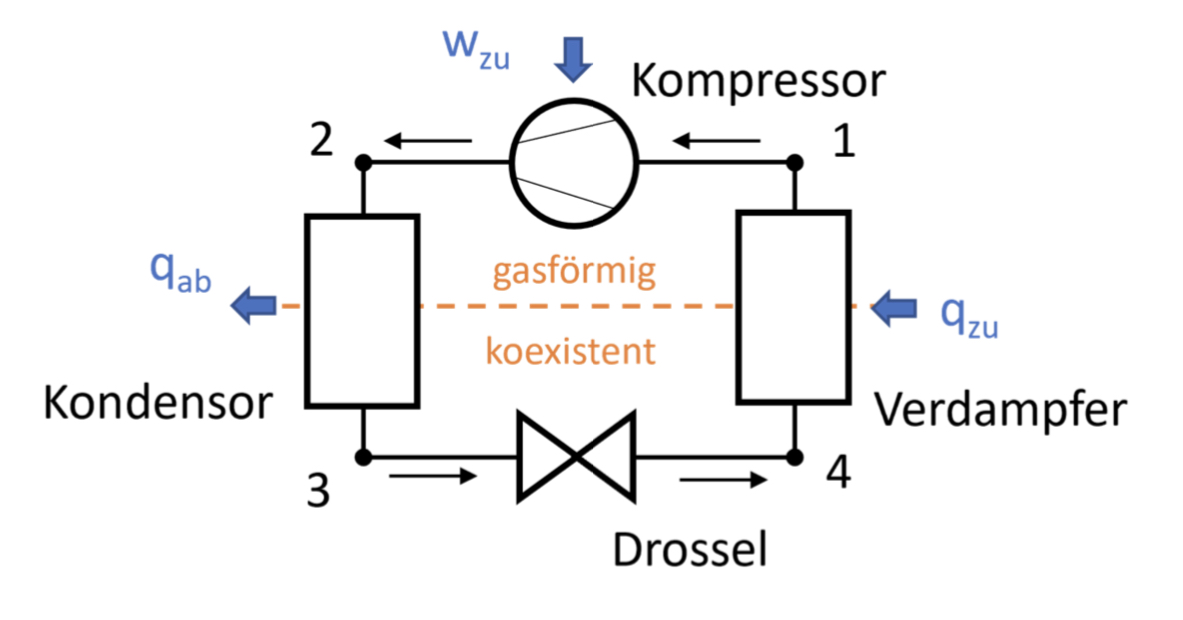
\includegraphics[width=0.8\textwidth]{images/Energiewissenschaften/Heat_pump.jpeg}
    \caption{Schema einer Wärmepumpe}
    \label{fig:heat_pump}
\end{figure} \\
Im ersten Schritt (1 $\rightarrow$ 2) wird mittels elektrischer Arbeit das gasförmige Arbeitsmittel im Kompressor verdichtet. Danach (2 $\rightarrow$ 3) kondensiert das Arbeitsmittel, dabei gibt es Wärme ab, aber seine Temperatur bleibt konstant. Anschließend (3 $\rightarrow$ 4) wird das Arbeitsmedium entspannt. Im finalen Schritt (4 $\rightarrow$ 1) wird das Arbeitsmittel unter Zugabe von Wärme bei konstanter Temperatur verdampft.\\  
\end{addmargin}
\newpage
\noindent\textbf{6. Wie lauten der energetische und exergetische Wirkungsgrad für eine reine elektrische Raumheizung?}\\
\begin{addmargin}[25pt]{0pt}     
Die Umgebungstemperatur sei $T_{\si{am}}$ während die Temperatur des Heizkörpers $T_{\si{H}}$ ist.\\ 
Der energetische Wirkungsgrad $\eta_1$ ist definiert als der Quotient aus eingehender und ausgehender Energie, da wir eine ideale elektrische Heizung annehmen ist dieser 100\%. Der exergetische Wirkungsgrad ist der Quotient von ausgehender Exergie und eingehender Exergie, die eingehende Exergie ist dabei die elektrische Energie $P_{\si{el}}$, da elektrische Energie reine Exergie ist. Die ausgehende Exergie ist die Wärmemenge die die Heizung zur Verfügung stellt (also auch die elektrische Energie $P_{\si{el}}$) multipliziert mit dem Carnot-Wirkungsgrad für eine Maschine die zwischen $T_{\si{am}}$ und $T_{\si{H}}$ arbeitet. Damit ergibt sich für typische Werte von $T_{\si{am}}$ und $T_{\si{H}}$:
\begin{align}\label{eq:eta1_elektroheizung}
    \eta_1 &= \frac{\dot{Q}}{P_{\si{el}}} = \frac{P_{\si{el}}}{P_{\si{el}}} = 100\% \\ \label{eq:eta2_elektroheizung}
    \eta_2 &= \frac{\Phi_{\si{out}}}{\Phi_{\si{in}}}=\frac{\dot{Q}\eta_c}{P_{\si{el}}} = \eta_c = \left( 1- \frac{T_{\si{am}}}{T_{\si{H}}}\right) \approx 15\%
\end{align}
Diesen Sachverhalt kann man auch gut in einem Energie- und Exergieflussdiagramm darstellen.
\begin{figure}[h]
    \centering
    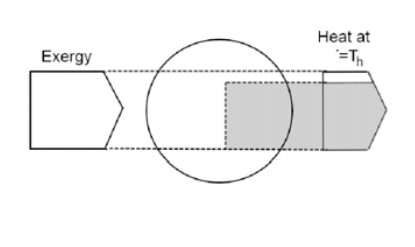
\includegraphics[width = 0.6\textwidth]{images/Energiewissenschaften/Exergiefluss_Elektroheizung.png}
    \caption{Energie- und Exergieflussdiagramm einer Elektroheizung. Der gesamte Pfeil zeigt die Energie wobei der graue Teil die Anergie und der weiße Teil die Exergie ist.}
    \label{fig:Exergeifluss_Elektroheizung}
\end{figure}\\
In Abbildung \ref{fig:Exergeifluss_Elektroheizung} kann man sehen wie keine Energie verloren geht, aber sehr viel Exergie in Anergie umgewandelt wird.\\
\end{addmargin}

\noindent\textbf{7. Wie lauten der energetische und exergetische Wirkungsgrad für eine Wärmepumpe?}\\
\begin{addmargin}[25pt]{0pt}     
Der exergetische Wirkungsgrad von einer Wärmepumpe ist $\eta_2 = 100\%$ da es sich um einen idealen reversiblen Prozess handelt. Der energetische Wirkungsgrad einer Wärmepumpe ist immer größer oder gleich 1, weil man ursprünglich nur eine geringe Menge Exergie in Form von elektrischer Energie hat und diese nutzt um eine große Menge Anergie von $T_{\si{am}}$ zu $T_{\si{H}}$ zu transportieren.\newpage
\begin{figure}[h]
    \centering
    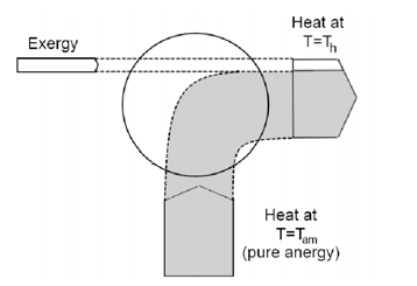
\includegraphics[width = 0.6\textwidth]{images/Energiewissenschaften/Exergiefluss_heat_pump.png}
    \caption{Energie- und Exergieflussdiagramm einer Wärmepumpe. Der gesamte Pfeil zeigt die Energie wobei der graue Teil die Anergie und der weiße Teil die Exergie ist.}
    \label{fig:Exergiefluss_heat_pump}
\end{figure}
\noindent Analog zum Fall der Elektroheizung kann man den Carnot-Wirkungsgrad nutzen um zu bestimmen wie viel Energie man maximal transportieren kann, es ergibt sich:
\begin{align}\label{eq:eta1_heat_pump}
    \eta_1 &= \frac{E_{\si{nutz}}}{E_{\si{in}}} = \frac{1}{\eta_c} \approx 670\% \\ \label{eq:eta2_heat_pump}
    \eta_2 &= \frac{\Phi_{\si{out}}}{\Phi_{\si{in}}}= 100\%
\end{align}

\end{addmargin}

\noindent\textbf{8. Sollte man sich eine Wärmepumpe oder eine rein elektrische Heizung bevorzugt einbauen?}\\
\begin{addmargin}[25pt]{0pt}     
Basierend auf den Wirkungsgraden aus den Gleichungen \ref{eq:eta1_elektroheizung}, \ref{eq:eta2_elektroheizung}, \ref{eq:eta1_heat_pump} und \ref{eq:eta2_heat_pump} ist die günsitgere Wahl die Wärmepumpe, da man bei ihr mit der gleichen Menge elektrischer Energie deutlich mehr Wärme transportieren kann. Außerdem wurde gesehen, dass bei Wärmepumpen kein Exergieverlust stattfindet, wohingegen die elektrische Heizung einen sehr hohen Exergieverlust aufweist. \\
\end{addmargin}

\noindent\textbf{9. Wärme wird von einem System zu einem anderen System transportiert. Der exergetische Wirkungsgrad für diesen Prozess lautet $\eta_2 =1$. Wie groß muss in diesem Fall die Temperaturdifferenz $\Delta T$ der beiden Systeme sein?}\\
\begin{addmargin}[25pt]{0pt}     
Wärmetransport zwischen zwei Systemen geht immer einher mit Exergieverlust, aufgrund des exergetischen Wirkungsgrades wissen wir dass bei dem beschriebenen Prozess keine Exergei verloren geht. Dies ist ein Widerspruch! Wir schlussfolgern daraus dass die beiden System im thermischen Gleichgewicht sein müssen, also gilt $\Delta T= 0$\\
\end{addmargin}

\noindent \textbf{10. Wie verhält sich der exergetische Wirkungsgrad beim Wärmetransport zwischen zwei Reservoirs für verschiedene zur Temperaturdifferenz proportionale Wärmeflussraten $\dot{Q}$ und Temperaturen der Reservoirs?}\\
\begin{addmargin}[25pt]{0pt}
    Der exergetische Wirkungsgrad hat die beiden Grenzfälle $\eta_2 = 1$ für $\dot{Q} = 0$ und $\eta_2 = 1- \frac{T_{\si{am}}}{T_2}$ für $\dot{Q} \rightarrow \infty$. Für einen gegebenen Wert von $\dot{Q}$ steigt der exergetische Wirkungsgrad mit den Temperaturen der Reservoirs. \\
\end{addmargin}

\noindent \textbf{11. Was ist der Unterschied zwischen einer elektrischen Wärmepumpe und einer Absorptionswärmepumpe?}\\
\begin{addmargin}[25pt]{0pt}
    Die elektrische Wärmepumpe nutzt elektrische Energie um den Kompressor zu betreiben, dabei wird also reine Exergie genutzt um Wärme von einem kalten Reservoir zu einem warmen zu pumpen. Die Absorptionswärmepumpe hingegen nutzt Wärme von einem noch heißeren Reservoir um den Kompressor anzutreiben. Man braucht bei beiden Systemen die gleiche Menge an Exergieinput allerdings ist bei der Absorptionswärmepumpe der Gesamtenergieinput größer als bei der elektrischen Wärmepumpe.\\
\end{addmargin}

\noindent \textbf{12. Ein Haus wird mit einer elektrischen Wärmepumpe geheizt welche mit einem perfekt isolierten Reservoir verbunden ist. Wie ändert sich die energetische Effizienz im Laufe der Zeit?}\\
\begin{addmargin}[25pt]{0pt}
    Aus Gleichung \ref{eq:eta1_heat_pump} wissen wir bereits wie der energetische Wirkungsgrad einer Wärmepumpe mit der Temperatur zusammenhängt. Nun müssen wir noch verstehen, dass das isolierte Reservoir aus der Aufgabe im Laufe der Zeit immer kälter wird, also die Temperatur $T_C$ sinkt. Umformen von Gleichung \ref{eq:eta1_heat_pump} ergibt: 
    \begin{equation}
        \eta_1 = \frac{1}{\eta_c} = \frac{T_{H}}{T_{H} - T_{C}}
    \end{equation}
    damit erkennt man, dass bei sinkendem $T_C$ der energetische Wirkungsgrad sich 1 annähert und somit sinkt. (Erinnerung: Er war vorher stets größer als 1)\\
\end{addmargin}

\noindent \textbf{13. Was ist der Unterschied zwischen einem geschlossenen und einem offenen System? Wie lautet jeweils der erste Haupsatz?}\\
\begin{addmargin}[25pt]{0pt}
Ein geschlossenes System kann mit der Umgebung nur Energie und keine Masse austauschen, wohingegen ein offenes System sowohl Masse als auch Energie austauschen kann. Der erste Hauptsatz der Thermodynamik lautet für geschlossene Systeme:
\begin{equation}\label{eq:1.HS_geschlossen}
    \si{d}U = \delta Q + \delta W
\end{equation}
dabei ist $U$ die innere Energie des Systems und $Q$ beziehungsweise $W$ die während eines Prozesses zugegebene/abgegebene Wärme beziehungsweise Arbeit.\\
Der erste Hauptsatz für offene Systeme ist etwas anders, da um den Massefluss aufrecht zu erhalten auch Arbeit benötigt wird, welche allerdings die innere Energie nicht beeinflusst. Der erste Hauptsatz für offene Systeme lautet dabei:
\begin{equation}\label{eq:1.HS_offen}
    \si{d}H = \delta Q + \delta W_t
\end{equation}
dabei ist $H = U + pV$ die Enthalpie und $W_t$ die Verschiebearbeit.\\
\end{addmargin}

\noindent \textbf{14. Wie ist die technische Arbeit definiert und was sagt diese aus?}\\
\begin{addmargin}[25pt]{0pt}
Die technische Arbeit ist in offenen Systemen der Teil der Gesamtarbeit, welcher nicht benötigt wird um die Masse durch das System zu drücken. Die Arbeit, welche gebraucht wird um den Massefluss aufrecht zu erhalten ist die dissipative Arbeit $W_{dis}$, es gilt:
\begin{equation}\label{eq:technische_Arbeit_dissipativ}
    W = W_t + W_{dis}
\end{equation}
Die technische Arbeit ist eine Prozessgröße die durch die Druckänderung des Arbeitsmediums charakterisiert wird, ihre Definition lautet:
\begin{equation}\label{eq:technische_Arbeit_Definition}
    \delta W_t = V\cdot \si{d}p
\end{equation}
\\
\end{addmargin}

\noindent \textbf{15. Aus welchen 4 Bestandteilen ist ein Dampfkraftwerk aufgebaut?}\\
\begin{addmargin}[25pt]{0pt}
Eine schematische Zeichnung eines Dampfkraftwerkes ist in Abbildung \ref{fig:Dampfkraftwerk} dargestellt. Das Dampfkraftwerk basiert auf dem Rankine-Zyklus. Dafür werden eine Pumpe, ein Verdampfer, eine Turbine und ein Kondensor benötigt. Die Pumpe komprimiert das flüssige Arbeitsmittel unter Zufuhr von Arbeit. Im Verdampfer wird das Arbeitsmittel unter Zugabe von Wärme verdampft. Danach gibt das Gas, welches immer noch unter hohem Druck steht, Arbeit in der Turbine ab, dadurch entspannt sich das Gas, die verrichtete Arbeit ist technische Arbeit. Schließlich wird im Kondensor das Gas wieder unter Abgabe von Wärme verflüssigt. Während dieses Prozesses geht im Kondensor am meisten Energie verloren, weil die abgegebene Wärme nicht weiter nutzbar ist in diesem Prozess. Allerdings geht die meiste Exergie im Verdampfer verloren, weil dabei Wärme von einem sehr warmen Reservoir auf das kältere Arbeitsmedium übertragen wird.\\
\begin{figure}[h]
    \centering
    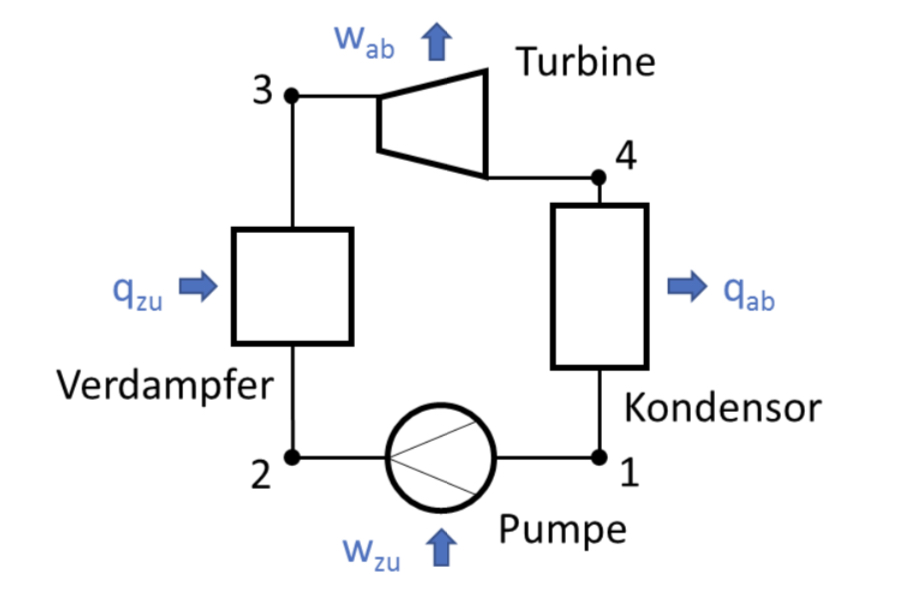
\includegraphics[width = 0.8\textwidth]{images/Energiewissenschaften/Dampfkraftwerk.jpeg}
    \caption{Schematische Zeichnung eines Dampfkraftwerkes}
    \label{fig:Dampfkraftwerk}
\end{figure}\\
\end{addmargin}

\noindent \textbf{16. Wie sieht der Rankine-Zyklus im $T$-$S$-Diagramm und wie im $p$-$V$-Diagramm aus? Was ergibt sich für den energetischen Wirkungsgrad?}\\
\begin{addmargin}[25pt]{0pt}
Von Zustand 1 zu 2 wird das flüssige Arbeitsmittel komprimiert, dabei ändert sich das Volumen kaum da es sich um eine inkompressible Flüssigkeit handelt, die Zufuhr von Arbeit resultiert lediglich in einer Steigerung des Drucks und der Temperatur. Danach wird das Arbeitsmedium isobar verdampft, man beachte dabei, dass der 2 Phasen-Bereich passiert wird und somit die Isobare im $T$-$S$-Diagramm einen Knick hat. Von Zustand 3 zu 4 wird technische Arbeit isentrop abgeführt und das Arbeitsmedium so entspannt. Schließlich wird unter Abfuhr von Wärme das Gas wieder kondensiert und in den Ausgangszustand gebracht. 
\begin{figure}[h]
    \centering
    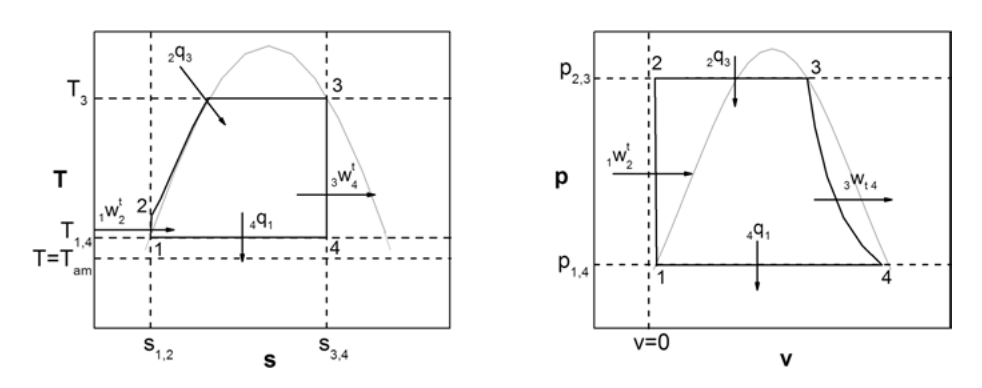
\includegraphics[width = 0.8\textwidth]{images/Energiewissenschaften/Rankinezyklus.png}
    \caption{$T$-$S$-Diagramm und $p$-$V$-Diagramm für den Rankine-Zyklus mit Phasenübergang}
    \label{fig:Rankinezyklus}
\end{figure}
Der energetische Wirkungsgrad ist in Gleichung \ref{eq:energetischer_Wirkungsgrad} definiert. Angewendet auf den Rankine-Zyklus ergibt das:
\begin{equation}\label{eq:Rankine_energetischer_Wirkungsgrad}
   \eta_1 = \frac{-(W_{t,12}-W_{t,34})}{Q_{23}} 
\end{equation}

\end{addmargin}

\noindent \textbf{17. Welche beiden Möglichkeiten gibt es den Wirkungsgrad eines realen Dampfkraftwerkes zu erhöhen?}\\
\begin{addmargin}[25pt]{0pt}
Die erste Möglichkeit ist die Zwischenüberhitzung, dabei wird der Dampf bei hohem Druck weiter erhitzt wodurch die Kondensation des Wassers erst nach der Turbine und nicht schon in der Turbine geschieht. Das ist hilfreich da Wasserdampf in der Turbine die Lebensdauer dieser erheblich verringert.\\ Die zweite Möglichkeit ist die Speisewasservorwärmung, dabei wird das in den Verdampfer geleitete Wasser mit Abwärme aus dem Wärmetauscher vorgewärmt wodurch sich der exergetische Wirkungsgrad erhöht.   \\
\end{addmargin}

\noindent \textbf{18. Wie funktioniert ein Gaskraftwerk?}\\
\begin{addmargin}[25pt]{0pt}
Bei einem Gaskraftwerk wird Luft bei Umgebungsbedingungen in einen Kompressor gespeist und dort adiabatisch auf einen höheren Druck gebracht. Danach wird dem Arbeitsgas Wärme isobar zugeführt, diese Wärme kommt aus den Verbrennungsgasen. In einer Turbine wird nun das Gas adiabatisch entspannt, dabei verrichtet es Arbeit. Das Gas wird nun an die Umgebung abgegeben wo es isobar abkühlt bis es die Umgebungsbedingungen erreicht hat. Das Gaskraftwerk basiert auf dem Joule-Brayton Zyklus, also 2 isobaren und 2 adiabatischen Zustandsänderungen. Anders als beim Dampfkraftwerk durchläuft das Gaskraftwerk keinen geschlossenen Kreislauf sondern einen offenen, es wird also immer neue Luft aus der Umgebung gezogen und am Ende des Zyklus wieder an die Umgebung abgegeben. Gaskraftwerke haben den Vorteil, dass sie ein kurze Startzeit haben und sehr gut regelbar sind, dadurch kann man sie sehr gut einsetzen um Schwankungen im Stromnetz zu kompensieren.\\
\end{addmargin}

\noindent \textbf{19. Nutzt man in der Realität eher Gas- oder eher Dampfkraftwerke?}\\
\begin{addmargin}[25pt]{0pt}
In der Realität nutzt man eine eine Hybridform aus Gas- und Dampfkraftwerk. Dabei werden die Abgase aus dem Gaskraftwerk genutzt um das Dampfkraftwerk anzutreiben. Reine Gaskraftwerke können einen Wirkungsgrad von $\eta_G = 30\%$ erreichen wohingegen Dampfkraftwerke $\eta_D = 40\% $ erreichen können, kombinierte Gas-Dampfkraftwerke erreichen aktuell einen Wirkungsgrad von $\eta_{GD} = 50\%$. Nutzt man das Gas-Dampfkraftwerk zusätzlich noch zur Einspeidung in das Fernwärmenetz so ist sogar ein wirkungsgrad von $\eta_{max} = 70\%$ möglich. \\
\end{addmargin}

\noindent \textbf{20. Wie hängt der energetische Wirkungsgrad und die nutzbare technische Arbeit von dem Druckverhältnis $\pi = \frac{p_{high}}{p_{low}}$ ab?}\\
\begin{addmargin}[25pt]{0pt}
Aus der Betrachtung der Energien im Joule-Brayton-Zyklus findet man für den energetischen Wirkungsgrad die Bedingung $\eta_{G} = 1 -\frac{T_1}{T_2}$. Setzt man darin nun die Bedingung für die adiabatischen Prozesse ein so findet man den energetischen Wirkungsgrad abhängig von den Drücken: 
\begin{align}
    \frac{T_4}{T_3} &= \left( \frac{p_4}{p_3}\right)^\frac{\kappa -1}{\kappa}= \frac{T_1}{T_2}\\
    \eta_G &= 1 - \frac{T_1}{T_2} = 1 - \left( \frac{p_4}{p_3}\right)^\frac{\kappa -1}{\kappa} = 1- \left( \frac{p_3}{p_4}\right)^{\frac{1}{\kappa} - 1} = 1- \pi^{\frac{1}{\kappa} - 1} 
\end{align}
Dabei ist $\kappa$ der Adiabatenkoeffizient. Man kann erkennen, dass der Wirkungsgrad umso größer wird je größer das Druckverhältnis ist, allerdings wird man bei Betrachtung der nutzbaren technischen Arbeit feststellen, dass genau an diesem Punkt man zwar einen hohen Wirkungsgrad aber eine geringe Leistung hat. Betrachtet man nun die nutzbare technische Arbeit und bestimmt bei welchem Druckverhältnis diese maximal ist so findet man ein ideales Druckverhältnis zum Betreiben des Gaskraftwerkes:
\begin{equation}\label{eq:ideales_Druckverhältnis_Gaskraftwerk}
    \pi_{w_tmax} = \left( \frac{T_3}{T_1}\right)^\frac{\kappa}{2(\kappa - 1)}
\end{equation}
Für dieses ideale Druckverhältnis ergibt sich ein Wirkungsgrad von:
\begin{equation}\label{eq:idealer_Wirkungsgrad_Gaskraftwerk}
\eta_{ideal} = 1 - \sqrt{\frac{T_1}{T_3}}    
\end{equation}
Außerdem gilt an diesem optimalen Arbeitspunkt $T_2 = T_4$.\\
\end{addmargin}

\subsection{Energieumwandlung von chemisch in elektrisch}
\noindent \textbf{1. Was ist die Aktivität eines Stoffes?}\\
\begin{addmargin}[25pt]{0pt}
Die Aktivität $a_k$ einer Spezies in einer Mischung ist ein dimensionsloses Maß der Konzentration. Bei der Aktivität werden die Wechselwirkungen zwischen den Molekülen mit berücksichtigt indem man einen Aktivitätskoeffizienten $f_k$ für die jeweilige Substanz mit inkludiert. Man kann das chemische Potential einer Spezies $\mu_k$ mit der Aktivität $a_k$ der Spezies ausdrücken:
\begin{equation}\label{eq:chemisches_Potential_Aktivität}
    \mu_k = \mu_k^0 + RT \ln a_k
\end{equation}
Hierbei ist $\mu_k^0$ das chemische Potential der reinen Substanz also mit $a_k = 1$.\\
\end{addmargin}

\noindent \textbf{2. Wie ist die Aktivität für (ideale) Gase, Flüssigkeiten, Ionen in Lösungen und Festkörper definiert?}\\
\begin{addmargin}[25pt]{0pt}
Für (ideale) Gase sind die Partialdrücke $p_k$ ein Maß für die Konzentration der einzelnen Bestandteile des Gasgemisches. Mit Berücksichtigung des Aktivitätskoeffizienten $f_k$ ergibt sich für die Aktivität einer Spezies: 
\begin{equation}\label{eq:activity_gas}
    a_{k,gas} = f_k \frac{p_k}{p_0}
\end{equation}
dabei ist $p_0$ der Gesamtdruck des Gasgemisches, heirfür wird fast immer der Druck bei Standardbedingungen also $1\; \si{atm} $ verwendet. Für ideale Gase ist $f_k = 1$.\\
In Flüssigkeiten beschreibt man die Konzentration mittels der Stoffmenge der Spezies dessen Aktivität man sucht $n_k$ und der Gesamtstoffmenge aller Flüssigkeiten in der Lösung $\sum\limits_j n_j$. Es ergibt sich die Aktivität der Spezies $k$ mit:
\begin{equation}\label{eq:activity_liquid}
    a_{k,liquid} = f_k \frac{n_k}{\sum\limits_j n_j}
\end{equation}
Bei Ionengemischen in einer Lösung nutzt man direkt die Konzentration $c_k$ der Spezies $k$ zur Bestimmung der Aktivität:
\begin{equation}\label{eq:activity_ions}
    a_{k,ion} = f_k\frac{c_k}{c_0}
\end{equation}
Dabei ist $c_0 = 1\si{M}$ die Konzentration bei Standardbedingungen (analog zum Fall mit Gasen).\\
Bei Festkörpern ist die Aktivität immer $a_k = 1$.\\
\end{addmargin}

\noindent\textbf{3. Wie ist die Exergie eines Brennstoffs bei vorgegebener chemischer Reaktion definiert? }\\
\begin{addmargin}[25pt]{0pt}
Die Exergie eines Brennstoffs ist die maximal nutzbare Arbeit durch Verbrauch des Brennstoffs über eine gegebene chemische Reaktion. Die Exergie entspricht damit dem Negativen der Änderung der Gibbs'schen Reaktionsenergie $G$:
\begin{equation}\label{eq:Exergie_chemische_Reaktion}
    \phi_k = -\Delta_rG
\end{equation}
Die Änderung der Gibbs'schen Reaktionsenergie hängt von der Aktivität der beteiligten Stoffe ab:
\begin{equation}\label{eq:Gibbs_Energie_activity}
    \Delta_rG = \Delta_rG^0 + RT \ln \left( \prod\limits_i a_i^{\nu_i}\right)
\end{equation}
Dabei ist $\nu_i$ der stöchiometrische Koeffizient der Spezies, er ist kleiner null für Edukte und größer null für Produkte. Bei der chemischen Reaktion:\\ 
\begin{center}
    \begin{large}
        \ce{CH4 + 2O2 -> CO2 + 2H2O}
    \end{large}
\end{center}
Ist der stöchiometrische Koeffizient $\nu$ für jeden Stoff gegeben mit:\\
$\nu_{\ce{CH4}} = -1$ \hspace{2cm} $\nu_{\ce{O2}} = -2$ \hspace{2cm} $\nu_{\ce{CO2}} = 1$ \hspace{2cm} $\nu_{\ce{H2O}} = 2$  \\
\end{addmargin}


\noindent\textbf{4. Wie findet man die Exergie wenn Energie in einer elektrochemischen Reaktion umgesetzt wird?}\\
\begin{addmargin}[25pt]{0pt}
Die Exergie bei einer elektrochemischen Reaktion ist gleich der Änderung der Gibbs-Energie $\Delta g_r^0$. Die Gibbs-Energie $G$ ist dabei definiert als 
\begin{equation}\label{eq:definition_Gibbs_Energie}
    G = H - TS
\end{equation}
Wobei $H$ die Enthalpie. $T$ die Temperatur und S die Entropie sind. Um bei einer bestimmten Reaktion die Exergie zu bestimmen muss man die tabellierten Werte für $H$ und $S$ der einzelnen beteiligten Stoffe verweden und kann damit die Gibbs-Energie bestimmen.\\
\end{addmargin}

\noindent\textbf{5. Was gilt für eine Redox-Reaktion an einer Grenzfläche?}\\
\begin{addmargin}[25pt]{0pt}
An der Grenzfläche zwischen Metall und Elektrolyt gleicht sich das elektrochemische Potential der Elektronen an. Dadurch können Elektronen zwischen Elektrolyt und Metall sich frei bewegen. Obwohl das elektrochemische Potential auf beiden Seiten der Grenzfläche gleich ist, so ist dennoch das elektrische Potential verschieden.\\
\end{addmargin}


\noindent\textbf{6. Was muss für die Elektroden-Überpotentiale gelten damit die Zellspannung einer galvanischen Zelle maximal ist?}\\
\begin{addmargin}[25pt]{0pt}
Die Elektroden-Überpotentiale an der Anode und an der Kathode haben unterschiedliche Vorzeichen damit der Elektronenfluss in die richtige Richtung gewährt werden kann. Die Überspannung an der Anode muss das Anodenpotential ein wenig in Richtung Kathode verschieben und bei der Kathode genau umgekehrt, dadurch wird die Zellspannung kleiner je größer die Überspannungen sind. Für eine möglichst große Zellspannung müssen die Beträge der Elektroden-Überspannungen also möglichst klein sein. Das kann man erreichen indem man einen Katalysator in die Zelle mit einbaut. \\
\end{addmargin}

\noindent\textbf{7. Wie ist die Standardzellspannung definiert und wie große ist sie in der Wasserstoffbrennzelle?}\\
\begin{addmargin}[25pt]{0pt}
Die Standardzellspannung $E^0$ ist über die Änderung der Gibbs-Energie pro mol $\Delta_rg^0$ definiert:
\begin{equation}\label{eq:def_Standardzellspannung}
    E^0 = -\frac{\Delta_rg^0}{nF}
\end{equation}
In dieser Gleichung steht $n$ für die Anzahl der an der Reaktion beteiligten Elektronen, das sind für die Wasserstoffbrennstoffzelle $n=4$. $F$ ist die Faraday-Konstante, sie gitb an wie viel Ladung ein Mol Elektronen tragen. Die Gibbs-Energie pro Mol ist gegeben als:
\begin{equation}\label{eq:gibbs_Brennstoffzelle}
    \Delta_rg^0 = \Delta_rh^0 - T\Delta_rs^0
\end{equation}
Für die gegebene Reaktion in der Brennstoffzelle:
\begin{center}
    \begin{large}
        \ce{ 2H2 + O2 -> 2H2O}
    \end{large}
\end{center}
kann nun mit den tabellierten Werten für die Reaktionsenthalpien $\Delta_rh^0$ und $\Delta_rs^0$ der einzelnen Reaktanten die gesamte Änderung der Gibbs-Energie während der Reaktion bestimmt werden. Man erhält $\Delta_rg^0 = -474,1 \;\frac{\si{kJ}}{\si{mol}}$ und damit eine Standardzellspannung von $E^0 = 1,23 \;\si{V}$\\
\end{addmargin}

\noindent\textbf{8. Wie ist der thermische Wirkungsgrad bei einer Wasserstoffbrennstoffzelle definiert und wie ändert er sich mit der Temperaatur?}\\
\begin{addmargin}[25pt]{0pt}
Der thermische Wirkungsgrad einer Wasserstoffbrennstoffzelle ist:
\begin{equation}\label{eq:thermischer_Wirkungsgrad_Brennstoffzelle}
    \eta_{th} = \frac{\Delta_rg^0}{\Delta_rh^0} 
\end{equation}
Diesen Ausdruck kann man mit Gleichung \ref{eq:gibbs_Brennstoffzelle} umformen, darin sieht man dann direkt die Temperaturabhängigkeit des Wirkungsgrades.
\begin{equation}
    \eta_{th} = \frac{\Delta_rh^0 - T\Delta_rs^0}{\Delta_rh^0} = 1- \frac{T\Delta_rs^0}{\Delta_rh^0}
\end{equation}
Das bedeutet der thermische Wirkungsgrad sinkt mit steigender Temperatur.
\end{addmargin}




\subsection{Energieumwandlung von solar in thermisch}
\subsection{Energieumwandlung von solar in elektrisch}

\noindent\textbf{1.}\\
\begin{addmargin}[25pt]{0pt}
Antwort\\
\end{addmargin}